\documentclass[11pt,a4paper]{report}
\usepackage[textwidth=37em,vmargin=30mm]{geometry}
\usepackage{calc,xunicode,amsmath,amssymb,paralist,enumitem,tabu,booktabs,datetime2,xeCJK,xeCJKfntef,listings}
\usepackage{tocloft,fancyhdr,tcolorbox,xcolor,graphicx,eso-pic,xltxtra,xelatexemoji}

\newcommand{\envyear}[0]{2025}
\newcommand{\envdatestr}[0]{2025-03-27}
\newcommand{\envfinaldir}[0]{webdb/2025/20250327/final}

\usepackage[hidelinks]{hyperref}
\hypersetup{
    colorlinks=false,
    pdfpagemode=FullScreen,
    pdftitle={Web Digest - \envdatestr}
}

\setlength{\cftbeforechapskip}{10pt}
\renewcommand{\cftchapfont}{\rmfamily\bfseries\large\raggedright}
\setlength{\cftbeforesecskip}{2pt}
\renewcommand{\cftsecfont}{\sffamily\small\raggedright}

\setdefaultleftmargin{2em}{2em}{1em}{1em}{1em}{1em}

\usepackage{xeCJK,xeCJKfntef}
\xeCJKsetup{PunctStyle=plain,RubberPunctSkip=false,CJKglue=\strut\hskip 0pt plus 0.1em minus 0.05em,CJKecglue=\strut\hskip 0.22em plus 0.2em}
\XeTeXlinebreaklocale "zh"
\XeTeXlinebreakskip = 0pt


\setmainfont{Brygada 1918}
\setromanfont{Brygada 1918}
\setsansfont{IBM Plex Sans}
\setmonofont{JetBrains Mono NL}
\setCJKmainfont{Noto Serif CJK SC}
\setCJKromanfont{Noto Serif CJK SC}
\setCJKsansfont{Noto Sans CJK SC}
\setCJKmonofont{Noto Sans CJK SC}

\setlength{\parindent}{0pt}
\setlength{\parskip}{8pt}
\linespread{1.15}

\lstset{
	basicstyle=\ttfamily\footnotesize,
	numbersep=5pt,
	backgroundcolor=\color{black!5},
	showspaces=false,
	showstringspaces=false,
	showtabs=false,
	tabsize=2,
	captionpos=b,
	breaklines=true,
	breakatwhitespace=true,
	breakautoindent=true,
	linewidth=\textwidth
}






\newcommand{\coverpic}[2]{
    % argv: itemurl, authorname
    Cover photo by #2~~(\href{#1}{#1})
}
\newcommand{\makeheader}[0]{
    \begin{titlepage}
        % \newgeometry{hmargin=15mm,tmargin=21mm,bmargin=12mm}
        \begin{center}
            
            \rmfamily\scshape
            \fontspec{BaskervilleF}
            \fontspec{Old Standard}
            \fontsize{59pt}{70pt}\selectfont
            WEB\hfill DIGEST
            
            \vfill
            % \vskip 30pt
            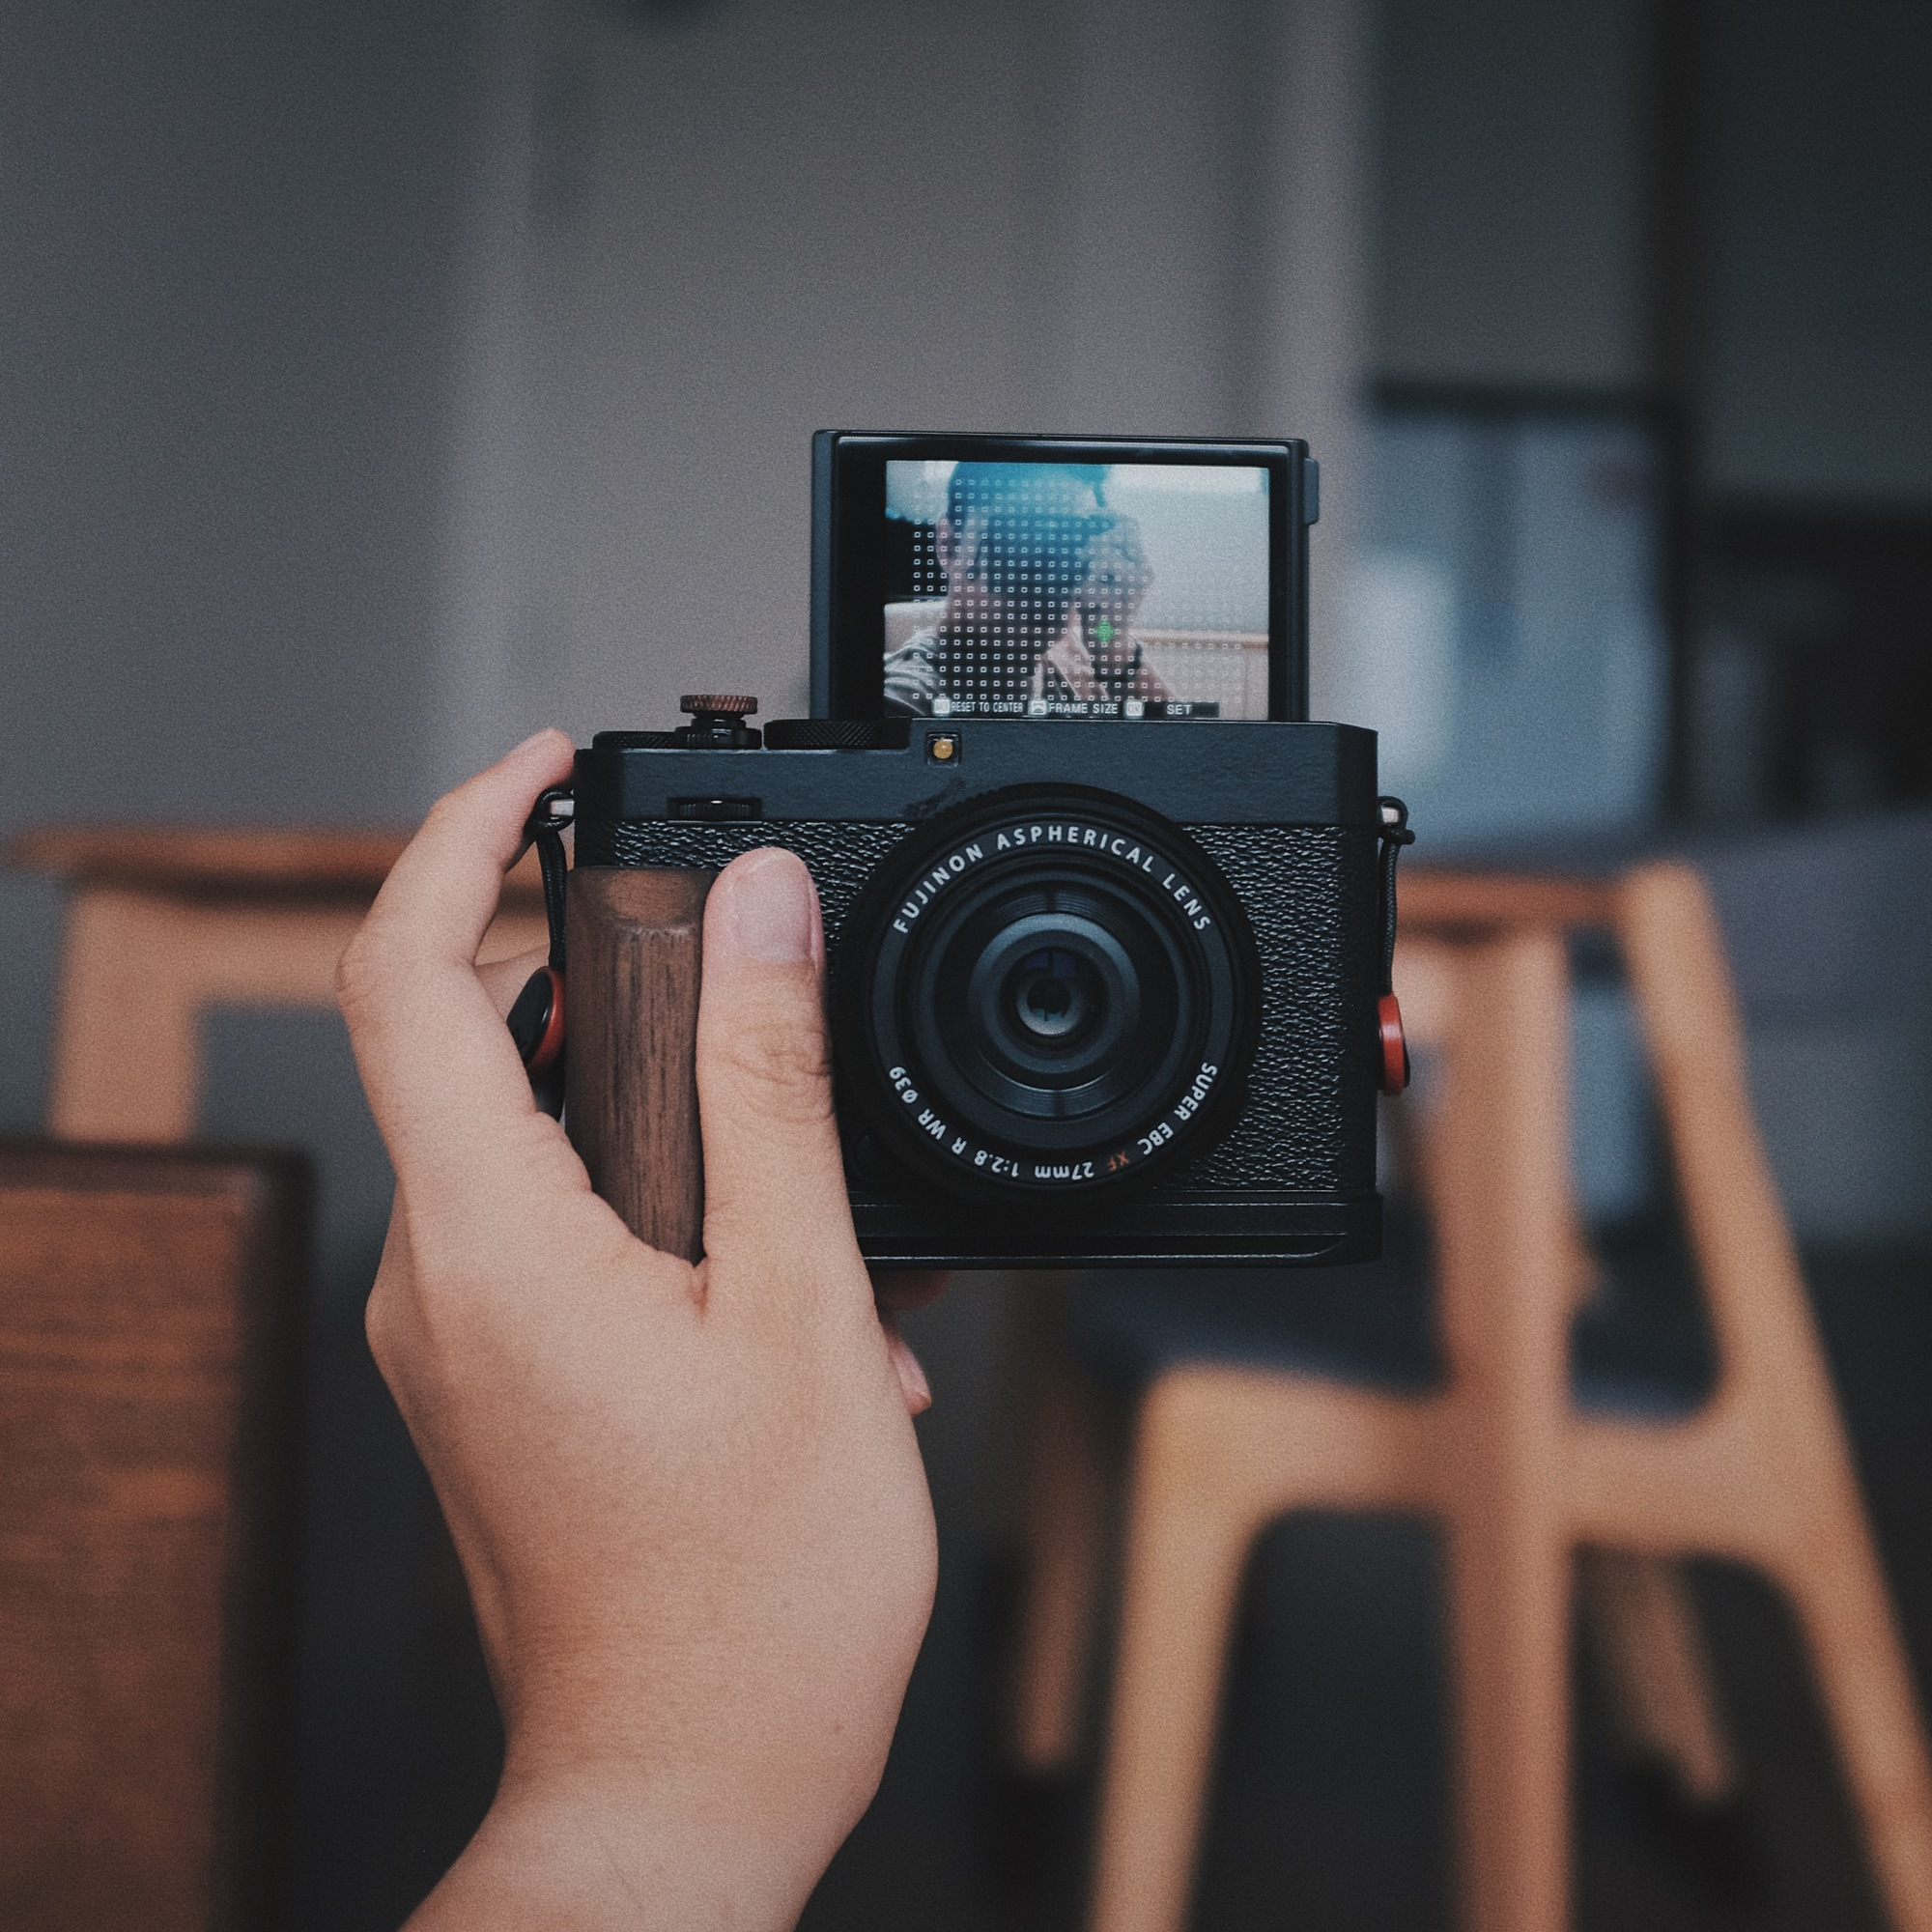
\includegraphics[width=\linewidth]{\envfinaldir/coverpic-prod.jpg}\par
            % \vskip 30pt
            \vfill

            \normalsize\rmfamily\scshape
            \copyright{} The Web Digest Project \hfill\large \envdatestr
        \end{center}
    \end{titlepage}
    % \restoregeometry
}
\newcommand{\simplehref}[1]{%
    \textcolor{blue!80!green}{\href{#1}{#1}}%
}
\renewcommand{\contentsname}{\center\Huge\sffamily\bfseries Contents\par\vskip 20pt}
\newcounter{ipartcounter}
\setcounter{ipartcounter}{0}
\newcommand{\ipart}[1]{
    % \vskip 20pt
    \clearpage
    \stepcounter{ipartcounter}
    \phantomsection
    \addcontentsline{toc}{chapter}{#1}
    % \begin{center}
    %     \Huge
    %     \sffamily\bfseries
    %     #1
    % \end{center}
    % \vskip 20pt plus 7pt
}
\newcounter{ichaptercounter}
\setcounter{ichaptercounter}{0}
\newcommand{\ichapter}[1]{
    % \vskip 20pt
    \clearpage
    \stepcounter{ichaptercounter}
    \phantomsection
    \addcontentsline{toc}{section}{\numberline{\arabic{ichaptercounter}}#1}
    \begin{center}
        \Huge
        \sffamily\bfseries
        #1
    \end{center}
    \vskip 20pt plus 7pt
}
\newcommand{\entrytitlefont}[1]{\subsection*{\raggedright\Large\sffamily\bfseries#1}}
\newcommand{\entryitemGeneric}[2]{
    % argv: title, url
    \parbox{\linewidth}{
        \entrytitlefont{#1}\par\vskip 5pt
        \footnotesize\ttfamily\mdseries
        \simplehref{#2}
    }\vskip 11pt plus 11pt minus 1pt
}
\newcommand{\entryitemGithub}[3]{
    % argv: title, url, desc
    \parbox{\linewidth}{
        \entrytitlefont{#1}\par\vskip 5pt
        \footnotesize\ttfamily\mdseries
        \simplehref{#2}\par\vskip 5pt
        \small\rmfamily\mdseries#3
    }\vskip 11pt plus 11pt minus 1pt
}
\newcommand{\entryitemAp}[3]{
    % argv: title, url, desc
    \parbox{\linewidth}{
        \entrytitlefont{#1}\par\vskip 5pt
        \footnotesize\ttfamily\mdseries
        \simplehref{#2}\par\vskip 5pt
        \small\rmfamily\mdseries#3
    }\vskip 11pt plus 11pt minus 1pt
}
\newcommand{\entryitemHackernews}[3]{
    % argv: title, hnurl, rawurl
    % \parbox{\linewidth}{
    %     \entrytitlefont{#1}\par\vskip 5pt
    %     \footnotesize\ttfamily\mdseries
    %     \simplehref{#3}\par
    %     \textcolor{black!50}{\href{#2}{#2}}
    % }\vskip 11pt plus 11pt minus 1pt
    \begin{minipage}{\linewidth}
            \entrytitlefont{#1}\par\vskip 5pt
            \footnotesize\ttfamily\mdseries
            \simplehref{#3}\par
            \textcolor{black!50}{\href{#2}{#2}}
    \end{minipage}\par\vskip 11pt plus 11pt minus 1pt
}







\begin{document}

\makeheader

\tableofcontents\clearpage




\ipart{Developers}
\ichapter{Hacker News}
\entryitemTwoLinks{Waymos crash less than human drivers}{https://news.ycombinator.com/item?id=43487231}{https://www.understandingai.org/p/human-drivers-keep-crashing-into}

\entryitemTwoLinks{Oracle customers confirm data stolen in alleged cloud breach is valid}{https://news.ycombinator.com/item?id=43486945}{https://www.bleepingcomputer.com/news/security/oracle-customers-confirm-data-stolen-in-alleged-cloud-breach-is-valid/}

\entryitemTwoLinks{How to Delete Your 23andMe Data}{https://news.ycombinator.com/item?id=43486236}{https://www.eff.org/deeplinks/2025/03/how-delete-your-23andme-data}

\entryitemTwoLinks{Google makes Android development private, will continue open source releases}{https://news.ycombinator.com/item?id=43485950}{https://arstechnica.com/gadgets/2025/03/google-makes-android-development-private-will-continue-open-source-releases/}

\entryitemTwoLinks{Playwright Tools for MCP}{https://news.ycombinator.com/item?id=43485740}{https://github.com/microsoft/playwright-mcp}

\entryitemTwoLinks{Airline Demand Between Canada and United States Collapses, Down 70\%+}{https://news.ycombinator.com/item?id=43485649}{https://onemileatatime.com/news/airline-demand-canada-united-states-collapses/}

\entryitemTwoLinks{Tufts student: Video shows masked agents arresting Rumeysa Ozturk}{https://news.ycombinator.com/item?id=43485577}{https://www.bostonglobe.com/2025/03/26/metro/tufts-student-video-shows-arrest/}

\entryitemTwoLinks{OpenAI adds MCP support to Agents SDK}{https://news.ycombinator.com/item?id=43485566}{https://openai.github.io/openai-agents-python/mcp/}

\entryitemTwoLinks{Google will develop Android OS behind closed doors starting next week}{https://news.ycombinator.com/item?id=43484927}{https://9to5google.com/2025/03/26/google-android-aosp-developement-private/}

\entryitemTwoLinks{Malware found on NPM infecting local package with reverse shell}{https://news.ycombinator.com/item?id=43484845}{https://www.reversinglabs.com/blog/malicious-npm-patch-delivers-reverse-shell}

\entryitemTwoLinks{Debian bookworm live images now reproducible}{https://news.ycombinator.com/item?id=43484520}{https://lwn.net/Articles/1015402/}

\entryitemTwoLinks{A love letter to the CSV format}{https://news.ycombinator.com/item?id=43484382}{https://github.com/medialab/xan/blob/master/docs/LOVE\_LETTER.md}

\entryitemTwoLinks{The Impact of Generative AI on Critical Thinking [pdf]}{https://news.ycombinator.com/item?id=43484224}{https://www.microsoft.com/en-us/research/wp-content/uploads/2025/01/lee\_2025\_ai\_critical\_thinking\_survey.pdf}

\entryitemTwoLinks{Good-bye core types; Hello Go as we know and love it}{https://news.ycombinator.com/item?id=43483842}{https://go.dev/blog/coretypes}

\entryitemTwoLinks{Botswana Successfully Launches First Satellite, Botsat-1}{https://news.ycombinator.com/item?id=43483660}{https://spaceinafrica.com/2025/03/15/botswana-successfully-launches-first-satellite-botsat-1/}

\entryitemTwoLinks{Linux kernel 6.14 is a big leap forward in performance and Windows compatibility}{https://news.ycombinator.com/item?id=43483567}{https://www.zdnet.com/article/linux-kernel-6-14-is-a-big-leap-forward-in-performance-and-windows-compatibility/}

\entryitemTwoLinks{Collapse OS}{https://news.ycombinator.com/item?id=43482705}{http://collapseos.org/}

\entryitemTwoLinks{Hyperlight WASM: Fast, secure, and OS-free}{https://news.ycombinator.com/item?id=43482556}{https://opensource.microsoft.com/blog/2025/03/26/hyperlight-wasm-fast-secure-and-os-free/}

\entryitemTwoLinks{Here are the Attack Plans That Trump's Advisers Shared on Signal}{https://news.ycombinator.com/item?id=43481521}{https://www.theatlantic.com/politics/archive/2025/03/signal-group-chat-attack-plans-hegseth-goldberg/682176/}

\entryitemTwoLinks{You should know this before choosing Next.js}{https://news.ycombinator.com/item?id=43481295}{https://eduardoboucas.com/posts/2025-03-25-you-should-know-this-before-choosing-nextjs/}\ichapter{Phoronix}
\entryitemGeneric{\hskip 0pt{}Linux 6.15 Adds Support For The New AMD Versal NET SoC}{https://www.phoronix.com/news/Linux-6.15-AMD-Versal-NET}

\entryitemGeneric{\hskip 0pt{}Microsoft Announces Open-Source "Hyperlight Wasm" Project}{https://www.phoronix.com/news/Microsoft-Hyperlight-Wasm}

\entryitemGeneric{\hskip 0pt{}Linux 6.15 Adds AMD Zen 5 SRSO Mitigation For KVM, Preps For Attack Vector Controls}{https://www.phoronix.com/news/Linux-6.15-x86-bugs}

\entryitemGeneric{\hskip 0pt{}Linux 6.15 Continues Improving Laptop Support}{https://www.phoronix.com/news/Linux-6.15-Laptop-Drivers}

\entryitemGeneric{\hskip 0pt{}Linux 6.15 Adds Raptor Lake-S Support To Intel EDAC Driver}{https://www.phoronix.com/news/Linux-6.15-EDAC}

\entryitemGeneric{\hskip 0pt{}AerynOS 2025.03 Released Following Rebrand From Serpent OS}{https://www.phoronix.com/news/AerynOS-2025.03-Linux}

\entryitemGeneric{\hskip 0pt{}KDE Developers Begin Working On A New Login Manager}{https://www.phoronix.com/news/KDE-New-Login-Manager-Over-SDDM}

\entryitemGeneric{\hskip 0pt{}IBM Says Goodbye To Cell Blade Servers With Linux 6.15}{https://www.phoronix.com/news/Linux-6.15-Dropping-Cell-Blades}

\entryitemGeneric{\hskip 0pt{}Intel Low Power Mode Daemon 0.0.9 Released For Linux Users}{https://www.phoronix.com/news/Intel-LPMD-0.0.9-Low-Power}\ichapter{Dribbble}
\entryitemGeneric{\hskip 0pt{}Proven UI/UX design, User Interface experience}{https://dribbble.com/shots/25819444-Proven-UI-UX-design-User-Interface-experience}

\entryitemGeneric{\hskip 0pt{}Dog + Play Button}{https://dribbble.com/shots/25809362-Dog-Play-Button}

\entryitemGeneric{\hskip 0pt{}Crypto Portfolio Tracker App}{https://dribbble.com/shots/25820014-Crypto-Portfolio-Tracker-App}

\entryitemGeneric{\hskip 0pt{}Illustration}{https://dribbble.com/shots/25822720-Illustration}

\entryitemGeneric{\hskip 0pt{}Gemini Rebrand}{https://dribbble.com/shots/25821410-Gemini-Rebrand}

\entryitemGeneric{\hskip 0pt{}Cyber Extrusion (Merch/Custom T-shirt)}{https://dribbble.com/shots/25821987-Cyber-Extrusion-Merch-Custom-T-shirt}

\entryitemGeneric{\hskip 0pt{}FCKD - Part 2}{https://dribbble.com/shots/25817864-FCKD-Part-2}

\entryitemGeneric{\hskip 0pt{}Aura - Logo Design}{https://dribbble.com/shots/25815819-Aura-Logo-Design}

\entryitemGeneric{\hskip 0pt{}Complexure}{https://dribbble.com/shots/25815646-Complexure}

\entryitemGeneric{\hskip 0pt{}Snitcher - New Branding}{https://dribbble.com/shots/25816140-Snitcher-New-Branding}

\entryitemGeneric{\hskip 0pt{}Lepisov Branding Logo Reveal Animation}{https://dribbble.com/shots/25814536-Lepisov-Branding-Logo-Reveal-Animation}

\entryitemGeneric{\hskip 0pt{}Spark illustrations}{https://dribbble.com/shots/25815705-Spark-illustrations}

\entryitemGeneric{\hskip 0pt{}Spark}{https://dribbble.com/shots/25815686-Spark}

\entryitemGeneric{\hskip 0pt{}FCKD}{https://dribbble.com/shots/25812257-FCKD}

\entryitemGeneric{\hskip 0pt{}Spark illustrations}{https://dribbble.com/shots/25815717-Spark-illustrations}

\entryitemGeneric{\hskip 0pt{}Revobyte Logo Design - R Letter / Monogram / Blockchain}{https://dribbble.com/shots/25811483-Revobyte-Logo-Design-R-Letter-Monogram-Blockchain}

\entryitemGeneric{\hskip 0pt{}Cimet Merch Car Wrapp}{https://dribbble.com/shots/25710572-Cimet-Merch-Car-Wrapp}

\entryitemGeneric{\hskip 0pt{}Task completion micro interaction}{https://dribbble.com/shots/25797132-Task-completion-micro-interaction}

\entryitemGeneric{\hskip 0pt{}Phantom auto buy/sell concept}{https://dribbble.com/shots/25799751-Phantom-auto-buy-sell-concept}

\entryitemGeneric{\hskip 0pt{}Lumee Logo Design - iGaming / Gambling / Casino}{https://dribbble.com/shots/25801924-Lumee-Logo-Design-iGaming-Gambling-Casino}

\entryitemGeneric{\hskip 0pt{}PurePaws - Logo Design}{https://dribbble.com/shots/25797575-PurePaws-Logo-Design}

\entryitemGeneric{\hskip 0pt{}S mark}{https://dribbble.com/shots/25796446-S-mark}

\entryitemGeneric{\hskip 0pt{}Central Coast}{https://dribbble.com/shots/25794367-Central-Coast}

\entryitemGeneric{\hskip 0pt{}The Sequencer Poster}{https://dribbble.com/shots/25798231-The-Sequencer-Poster}


\ipart{Developers~~~~(zh-Hans)}
\ichapter{Solidot}
\entryitemGeneric{\hskip 0pt{}比亚迪 2024 年销售收入超过特斯拉}{https://www.solidot.org/story?sid=80892}

\entryitemGeneric{\hskip 0pt{}火星发现长链有机分子}{https://www.solidot.org/story?sid=80891}

\entryitemGeneric{\hskip 0pt{}年轻一代的消费者更爱内容创作者而非传统电视电影}{https://www.solidot.org/story?sid=80889}

\entryitemGeneric{\hskip 0pt{}近半加拿大家庭完全停止消费有线电视}{https://www.solidot.org/story?sid=80888}

\entryitemGeneric{\hskip 0pt{} Infinite Reality 以 2.07 亿美元收购 Napster}{https://www.solidot.org/story?sid=80887}

\entryitemGeneric{\hskip 0pt{}H5N1 禽流感在英国传播到绵羊}{https://www.solidot.org/story?sid=80886}

\entryitemGeneric{\hskip 0pt{}火星东半球被认为蕴含丰富的冰}{https://www.solidot.org/story?sid=80885}

\entryitemGeneric{\hskip 0pt{}交通噪音会触发鸟类的路怒症}{https://www.solidot.org/story?sid=80884}

\entryitemGeneric{\hskip 0pt{}东京法庭下令解散统一教会}{https://www.solidot.org/story?sid=80883}

\entryitemGeneric{\hskip 0pt{}Game Informer 杂志复活}{https://www.solidot.org/story?sid=80882}

\entryitemGeneric{\hskip 0pt{}李开复称中美 AI 差距仅为三个月}{https://www.solidot.org/story?sid=80881}

\entryitemGeneric{\hskip 0pt{}科学家寻求更精确的测量疼痛}{https://www.solidot.org/story?sid=80880}

\entryitemGeneric{\hskip 0pt{}银河系中心的龙卷风}{https://www.solidot.org/story?sid=80879}

\entryitemGeneric{\hskip 0pt{}如何减少 AI 大模型的功耗}{https://www.solidot.org/story?sid=80878}

\entryitemGeneric{\hskip 0pt{}2024 年全球气候多项指标创下记录}{https://www.solidot.org/story?sid=80877}

\entryitemGeneric{\hskip 0pt{}家族企业表现出更多环境责任行为}{https://www.solidot.org/story?sid=80876}

\entryitemGeneric{\hskip 0pt{}最新观测挑战宇宙标准模型}{https://www.solidot.org/story?sid=80875}

\entryitemGeneric{\hskip 0pt{}Google 和计算机历史博物馆发布 AlexNet 源代码}{https://www.solidot.org/story?sid=80874}

\entryitemGeneric{\hskip 0pt{}中国依靠工程师红利挑战美国的科技主导地位}{https://www.solidot.org/story?sid=80873}

\entryitemGeneric{\hskip 0pt{}FaunaDB 倒闭,计划开源}{https://www.solidot.org/story?sid=80872}\ichapter{V2EX}
\entryitemGeneric{\hskip 0pt{}[汽车] 双车道左转,被追尾我全责}{https://www.v2ex.com/t/1121365}

\entryitemGeneric{\hskip 0pt{}[问与答] 家庭中用 minio 是什么场景?}{https://www.v2ex.com/t/1121364}

\entryitemGeneric{\hskip 0pt{}[问与答] 目前``联网搜索''能力最强的 AI 目前是哪个? DeepSeek 吗?}{https://www.v2ex.com/t/1121363}

\entryitemGeneric{\hskip 0pt{}[程序员] 小型项目起步求助}{https://www.v2ex.com/t/1121362}

\entryitemGeneric{\hskip 0pt{}[问与答] 在实战中哪个 ai 解决问题, BUG 能力强啊}{https://www.v2ex.com/t/1121361}

\entryitemGeneric{\hskip 0pt{}[Apple] Mac - Lumon Terminal Pro}{https://www.v2ex.com/t/1121360}

\entryitemGeneric{\hskip 0pt{}[OpenWrt] 目前好像感受到了 openwrt 作为主路由的无力感}{https://www.v2ex.com/t/1121359}

\entryitemGeneric{\hskip 0pt{}[分享发现] 分享一个纯净版 AI Chat UI}{https://www.v2ex.com/t/1121357}

\entryitemGeneric{\hskip 0pt{}[问与答] Mac 窗口失焦、无法操作的问题}{https://www.v2ex.com/t/1121356}

\entryitemGeneric{\hskip 0pt{}[问与答] 最佳调 prompt 实践是什么?}{https://www.v2ex.com/t/1121355}

\entryitemGeneric{\hskip 0pt{}[健康] 新冠真的不是感冒}{https://www.v2ex.com/t/1121353}

\entryitemGeneric{\hskip 0pt{}[问与答] outlook 和 Gmail 不能像 QQ 和 iCloud 邮箱那样,可以把发件人和账户设置为不同的名称?}{https://www.v2ex.com/t/1121352}

\entryitemGeneric{\hskip 0pt{}[Android] 2025 年了,三星插 sim 卡送中还是无解吗}{https://www.v2ex.com/t/1121351}

\entryitemGeneric{\hskip 0pt{}[程序员] V2er 都是怎么使用大模型 api 的呢,想在命令行使用 api,有没有好用的 api 命令行工具呢 就是一轮会话后自动进入下一轮}{https://www.v2ex.com/t/1121350}

\entryitemGeneric{\hskip 0pt{}[分享发现] 美的洗碗机一周偷跑 200G 流量}{https://www.v2ex.com/t/1121349}

\entryitemGeneric{\hskip 0pt{}[问与答] 大家的大脑是单核的还是多核的?}{https://www.v2ex.com/t/1121348}

\entryitemGeneric{\hskip 0pt{}[问与答] Chrome 的光标 bug}{https://www.v2ex.com/t/1121347}

\entryitemGeneric{\hskip 0pt{}[问与答] 大厂生存之道卷是最基础的吗?}{https://www.v2ex.com/t/1121346}

\entryitemGeneric{\hskip 0pt{}[酷工作] 25 届应届生求职问题,虚心求教}{https://www.v2ex.com/t/1121345}

\entryitemGeneric{\hskip 0pt{}[Go 编程语言] ai 对话内容如何持久化}{https://www.v2ex.com/t/1121344}

\entryitemGeneric{\hskip 0pt{}[投资] 标普 500 指数到底是个啥玩意儿?}{https://www.v2ex.com/t/1121343}

\entryitemGeneric{\hskip 0pt{}[问与答] 关于 Go 并发获取数据的问题,请教大家}{https://www.v2ex.com/t/1121341}

\entryitemGeneric{\hskip 0pt{}[程序员] 为 GoldenDict 中添加 AI 词典}{https://www.v2ex.com/t/1121339}

\entryitemGeneric{\hskip 0pt{}[问与答] 咨询下,多年欠款下除了债务重组是否有其他方案}{https://www.v2ex.com/t/1121338}

\entryitemGeneric{\hskip 0pt{}[macOS] 坏消息: Setapp 取消家庭计划}{https://www.v2ex.com/t/1121336}

\entryitemGeneric{\hskip 0pt{}[分享创造] 有人对中医气血数字化感兴趣的吗}{https://www.v2ex.com/t/1121335}

\entryitemGeneric{\hskip 0pt{}[问与答] 买的国外代理 ip,有什么方法能在国内的网络使用吗?}{https://www.v2ex.com/t/1121333}

\entryitemGeneric{\hskip 0pt{}[Linux] 分享一个 Linux 下的改键工具}{https://www.v2ex.com/t/1121332}

\entryitemGeneric{\hskip 0pt{}[硬件] 想做个远程控制设备,有没有大佬指导下}{https://www.v2ex.com/t/1121331}

\entryitemGeneric{\hskip 0pt{}[分享创造] 做 Youtube 视频的几个月,我的真实收入情况}{https://www.v2ex.com/t/1121330}

\entryitemGeneric{\hskip 0pt{}[分享创造] 试了试今天的 deepseek V3 0325,做了一个多语言站点}{https://www.v2ex.com/t/1121329}

\entryitemGeneric{\hskip 0pt{}[iOS] ios18 音量不能细调了吗}{https://www.v2ex.com/t/1121328}

\entryitemGeneric{\hskip 0pt{}[程序员] Lark/飞书 开发 bot 完偶然发现视频/投屏开始收费了}{https://www.v2ex.com/t/1121327}

\entryitemGeneric{\hskip 0pt{}[生活] 有自己买养老保险的吗,值得买吗?}{https://www.v2ex.com/t/1121326}

\entryitemGeneric{\hskip 0pt{}[旅行] 三天两晚,济州岛游记}{https://www.v2ex.com/t/1121325}

\entryitemGeneric{\hskip 0pt{}[macOS] 求推荐 MacOS HyperKey 方案}{https://www.v2ex.com/t/1121324}

\entryitemGeneric{\hskip 0pt{}[Apple] Mac mini, iMac}{https://www.v2ex.com/t/1121323}

\entryitemGeneric{\hskip 0pt{}[加密货币] Bybit 卡在日本旅游时的可用性}{https://www.v2ex.com/t/1121321}

\entryitemGeneric{\hskip 0pt{}[分享发现] 以后每次重装系统要做的事情又多了一个,微信居然可以设置使用默认浏览器打开网页!折磨我太久了}{https://www.v2ex.com/t/1121320}

\entryitemGeneric{\hskip 0pt{}[旅行] 问问见多识广的大佬,人生有必去的地方吗,不限国内外}{https://www.v2ex.com/t/1121319}

\entryitemGeneric{\hskip 0pt{}[京东] 兄弟们,京东上买五粮液和去线下买有什么区别吗?}{https://www.v2ex.com/t/1121317}

\entryitemGeneric{\hskip 0pt{}[上海] 种植牙如何选择?私立 or 公立,非常纠结,求助}{https://www.v2ex.com/t/1121316}

\entryitemGeneric{\hskip 0pt{}[生活] 有一个没有投资脑子爱投资的家人该咋办}{https://www.v2ex.com/t/1121314}

\entryitemGeneric{\hskip 0pt{}[Android] 请问各位大佬 Android 13 未 root 情况下,可以调用 Wifiserviceimpl 的私有类吗?}{https://www.v2ex.com/t/1121313}

\entryitemGeneric{\hskip 0pt{}[互联网] 小红书上的独立开发都是小丑}{https://www.v2ex.com/t/1121311}

\entryitemGeneric{\hskip 0pt{}[编程] nextjs 能把人逼疯}{https://www.v2ex.com/t/1121309}

\entryitemGeneric{\hskip 0pt{}[职场话题] [选 Offer] BOSE VS 大宇无限}{https://www.v2ex.com/t/1121308}

\entryitemGeneric{\hskip 0pt{}[职场话题] 分享外包踩坑经历}{https://www.v2ex.com/t/1121307}

\entryitemGeneric{\hskip 0pt{}[分享创造] 一个 Dify Java 客户端}{https://www.v2ex.com/t/1121306}

\entryitemGeneric{\hskip 0pt{}[分享创造] 分享一个基于 WebRTC 的信息传输工具,另外求一份远程全栈工作}{https://www.v2ex.com/t/1121305}


\ipart{Generic News}
\ichapter{AP News}
\entryitemWithDescription{\hskip 0pt{}Will Smith gets street named in Philadelphia neighborhood where he was born and raised}{https://apnews.com/article/b84d2f19e88b9015c801d5ad59f2c673}{}

\entryitemWithDescription{\hskip 0pt{}30 years after music icon Selena's murder, Yolanda Saldívar is up for parole. Here's what to know}{https://apnews.com/article/c68df5e4f1e6398a54587044f35e652e}{}

\entryitemWithDescription{\hskip 0pt{}World Series champion LA Dodgers say they'll visit Trump at the White House on April 7}{https://apnews.com/article/fcf01550c4aee53039aa82fc88a7fe31}{}

\entryitemWithDescription{\hskip 0pt{}A new Chili's near Scranton will be a throwback to `The Office,' `awesome blossom' and all}{https://apnews.com/article/2faea0e7841dcd6903a798064fd17508}{}

\entryitemWithDescription{\hskip 0pt{}Pilot and 2 young daughters survive the night on airplane wing after crashing into icy Alaska lake}{https://apnews.com/article/f385057ebd03c32cd6d766d2c521e856}{}

\entryitemWithDescription{\hskip 0pt{}It was bacteria — not a miracle — on a Communion wafer in Indiana church}{https://apnews.com/article/fb90923979d6048dfacbacb65f11783f}{}

\entryitemWithDescription{\hskip 0pt{}Escaped otters cavort in the snow as the zoo's search continues}{https://apnews.com/article/937ee002eeced882e96b93ba36f16874}{}

\entryitemWithDescription{\hskip 0pt{}A new Trump portrait for Colorado's Capitol could take time after one he disliked was removed}{https://apnews.com/article/c10a3288cf2a6d5260e385265a066773}{}

\entryitemWithDescription{\hskip 0pt{}Napster sold to tech commerce company for \$207 million}{https://apnews.com/article/7c2541f805d8debf0433171696c54518}{}

\entryitemWithDescription{\hskip 0pt{}Utah adds protections for child influencers following YouTuber Ruby Franke's child abuse conviction}{https://apnews.com/article/d9702b22c9ea7adba6e15003971493ce}{}

\entryitemWithDescription{\hskip 0pt{}Texas Rep. Jasmine Crockett mocks Greg Abbott, who uses a wheelchair, as `Gov. Hot Wheels'}{https://apnews.com/article/a38d50b41e35cc6e05f5d72ad74ff54f}{}

\entryitemWithDescription{\hskip 0pt{}Kroger blames Albertsons for merger's demise in new court filings}{https://apnews.com/article/a93ae5b43e705c5350695c071a06331f}{}

\entryitemWithDescription{\hskip 0pt{}Waymo plans to bring its driverless taxis to Washington in 2026}{https://apnews.com/article/599b6323af61bad08e2ad6f27fca1102}{}






\clearpage
\leavevmode\vfill
\footnotesize

Copyright \copyright{} 2023-2025 Neruthes and other contributors.

This document is published with CC BY-NC-ND 4.0 license.

The entries listed in this newsletter may be copyrighted by their respective creators.

This newsletter is generated by the Web Digest project.

The newsletters are also delivered via Telegram channel \CJKunderline{\href{https://t.me/webdigestchannel}{https://t.me/webdigestchannel}}.\\
RSS feed is available at \CJKunderline{\href{https://webdigest.pages.dev/rss.xml}{https://webdigest.pages.dev/rss.xml}}.

This newsletter is available in PDF at
\CJKunderline{\href{https://webdigest.pages.dev/}{https://webdigest.pages.dev/}}.

The source code being used to generate this newsletter is available at\\
\CJKunderline{\href{https://github.com/neruthes/webdigest}{https://github.com/neruthes/webdigest}}.

This newsletter is also available in
\CJKunderline{\href{http://webdigest.pages.dev/readhtml/\envyear/WebDigest-20250327.html}{HTML}} and
\CJKunderline{\href{https://github.com/neruthes/webdigest/blob/master/markdown/\envyear/WebDigest-20250327.md}{Markdown}}.


\coverpic{https://unsplash.com/photos/a-person-riding-skis-down-a-snow-covered-slope-bLxT-7cQHxc}{Simon Takatomi}


\end{document}
